%%%% ijcai19.tex

\typeout{IJCAI-19 Instructions for Authors}

% These are the instructions for authors for IJCAI-19.

\documentclass{article}
\pdfpagewidth=8.5in
\pdfpageheight=11in
% The file ijcai19.sty is NOT the same than previous years'
\usepackage{ijcai19}

% Use the postscript times font!
\usepackage{times}
\usepackage{soul}
\usepackage{url}
\usepackage[hidelinks]{hyperref}
\usepackage[utf8]{inputenc}
\usepackage[small]{caption}
\usepackage{graphicx}
\usepackage{amsmath}
\usepackage{booktabs}
\usepackage{algorithm}
\usepackage{algorithmic}
% \usepackage{epstopdf}
\usepackage{makecell}
\usepackage{float}
\urlstyle{same}

% the following package is optional:
%\usepackage{latexsym}

% Following comment is from ijcai97-submit.tex:
% The preparation of these files was supported by Schlumberger Palo Alto
% Research, AT\&T Bell Laboratories, and Morgan Kaufmann Publishers.
% Shirley Jowell, of Morgan Kaufmann Publishers, and Peter F.
% Patel-Schneider, of AT\&T Bell Laboratories collaborated on their
% preparation.

% These instructions can be modified and used in other conferences as long
% as credit to the authors and supporting agencies is retained, this notice
% is not changed, and further modification or reuse is not restricted.
% Neither Shirley Jowell nor Peter F. Patel-Schneider can be listed as
% contacts for providing assistance without their prior permission.

% To use for other conferences, change references to files and the
% conference appropriate and use other authors, contacts, publishers, and
% organizations.
% Also change the deadline and address for returning papers and the length and
% page charge instructions.
% Put where the files are available in the appropriate places.

\title{ImageNet-trained CNNs are biased towards texture; increasing shape bias improves accuracy and robustness}

% Single author syntax
\iffalse
\author{
    Sarit Kraus
    \affiliations
    Department of Computer Science, Bar-Ilan University, Israel \emails
    pcchair@ijcai19.org
}
\fi

% Multiple author syntax (remove the single-author syntax above and the \iffalse ... \fi here)
% Check the ijcai19-multiauthor.tex file for detailed instructions

\author{
Andre Diler$^1$
\and
Mehdi Chaid$^1$\and
Abderahmane Bouziane$^1$\
\affiliations
$^1$Département GIGL Polytechnique Montreal\\
\emails
andre.diler@polymtl.ca,
mehdi.chaid@polymtl.ca,
abderahmane.bouziane@polymtl.ca
}

\begin{document}

\maketitle

\begin{abstract}
The history of computer vision led us to believe that like humans, 
Convolutional Neural Networks (CNNs) would recognize objects mainly by their shapes.
Recent studies in the field however, have  suggested that CNNs rely more on image textures 
rather than edges and shapes in order to perform object detection. 
A paper published in November 2018, by \cite{geirhos2018imagenettrained}, explored the idea of texture bias
and presented novels solutions in order to shift the trend towards a stronger shape bias for CNNs, similar to 
how humans perceive things.
The following report attempts to analyse the hypothesis proposed in the paper, 
as well as offer a scoped reproduction of the experiments conducted by the authors, in a smaller environment, 
in order to draw new conclusions and reinforce our understanding of the internals of CNNs.
\end{abstract}

\section{Introduction}

% https://hackernoon.com/a-brief-history-of-computer-vision-and-convolutional-neural-networks-8fe8aacc79f3

Modern Convolutional Neural Networks regularly reach very high performances on complex computer vision tasks 
such as image classification and segmentation.
These performances are reaching human levels in term of accuracy, and come from a long history of studies 
on human and machine perception. \medskip \par 

\noindent
As such, and reinforced with other experiments on the matter, 
it is commonly believed that CNNs learn features from the shapes during the training phase
and use these for detection.

\subsection{Related Work}

\noindent
The first proof that shapes are fundamental in computer vision came from a very influential study on cognition, 
by \cite{hubel1959receptive}, who described how biological neurons could extract features from images,
amongst which certain types of neurons were activated specifically by edges. \medskip \par 

\noindent 
Another paper from \cite{marr1982vision} concluded that vision was hierachical. Low-level features, such as lines,
were combined together to recognize more high level concepts, 
like wheels, windows, etc, and form objects. \medskip \par 

\noindent
The famous Neocognition paper \cite{neocognitron} was 
the implementation that introduced the idea of hierachical vision. 

\noindent
The multilayered neural network they proposed 
included multiple convolutional layers with wheighted receptive fields (filters).
It was the first known deep neural network. \medskip \par

\noindent
However, the first modern convnet was LeNet \cite{Lecun98gradient-basedlearning}.
This CNN used backpropagation to automatically learn the filter values to extract meaningful 
features in images hierachically.
Nowadays, all the recent convolutional neural networks are inspired from this network. \medskip \par

\noindent
ConvNet were considered like a black box for a long time, 
resulting in considerable efforts made in
recent years to analyze the inside of these networks. \medskip \par

\noindent
The shape hypothesis that emerged from early experiments consists in
"High-level units appear to learn representations of shapes occurring in natural images” 
\cite{Kriegeskorte029876}. This theory quickly became widespread in the community, and
is understandable given the history of computer vision. \medskip \par

\noindent
Furthermore, there are a lot of studies comparing human vision with computer vision. For example,
\cite{kubiliusshape} stated that 
"implicitly learn representations of shape that reflect human shape perception"
while a paper from \cite{ritter2017cognitive} concluded that 
"state-of-the-art one-shot learning models trained on ImageNet exhibit  
a similar bias to that observed in humans: they prefer to categorize objects according  
to shape rather than color" . \medskip \par

\noindent
However, several researchers raised doubts about the shape hypothesis.
According to studies from \cite{gatys2017textures} and \cite{brendel2019approximating}, 
CNNs are able to classify texturized images even if their shape structure is destroyed.
Moreover, the same paper from \cite{brendel2019approximating} also
showed that CNNs with constrained receptive field sizes can reach competitive accuracies on ImageNet.
It is also worth noticing that small receptive fields cannot capture the overal shape of an image.
These results have led the authors of the paper we've analysed, \cite{geirhos2018imagenettrained}, 
to emit a new hypothesis: the texture hypothesis, where "in contrast to the
common assumption, object textures are more important than global object shapes for CNN object
recognition". \medskip \par

\bigskip

Our objective in this report is to submit those hypothesis to a test through diverse experiments 
and validate the results obtained by the original authors in our own environment .

\newpage
\section{Methodology}

\subsection{Dataset}

We used Imagenette \cite{fastai2019}, a subset of the Imagenet dataset created 
by fastai to conduct our experiments.
This ensured that our results would be comparable to the authors, 
while keeping an acceptable size for the dataset given the time and material constraints.
Imagenette contains 13394 images.
Imagenette's train/test split is 70/30: 9469 images for the train and validation set, and 3925 images for the test set.
It contains 10 easily classifiable classes from Imagenet, namely
\textit{tench, English springer, cassette player, chain saw, church, 
French horn, garbage truck, gas pump, golf ball, parachute}.
The classes are balanced with around 950 images in each one. \smallskip \par
\vspace{-0.3cm}
\noindent
This dataset is more easily classifiable than Imagenet in less time, which fits our purpose.
We used the '160px' version of the images, where the shortest size of the images are resized to that size, 
with their aspect ratio maintained.

\subsection{Style Transfer}
\label{2.2-style-transfer}

This procedure ensures that the images conserve their edges, but not their textures.
In order to destroy all the texture information of an image without its edges, we used style transfer like in
the original paper.
However, we generated our own Stylized-Dataset. \medskip \par

\noindent
The image for which you want to change the texture, but keep the edges is called the \textbf{content image}.
The image were the the texture is extracted is called the \textbf{texture image}.
The image created by the style transfer is called the \textbf{stylized image}. \medskip \par

\noindent
We applied style transfer on Imagenette to replace the original texture of the object (dog's fur for example) 
with a random texture (a parachute's fabric and color) 
from sampled from the Describable Texture Dataset \cite{cimpoi14describing}. \medskip \par

\noindent
Our first aproach was to use a random image from the Texture Dataset to stylize Imagenette. However, 
the edges of the images were sometimes destroyed, and were not identifiable by humans. \medskip \par

\noindent
To avoid poor quality images, we handpicked 11 texture images that generated good quality stylized images.
Each time an Imagenette image was to be stylized, we picked a texture image randomly from our 11 textures.
This ensured that the texture of a stylized image had no correlation with its original class. \medskip \par

\noindent
We used the implementation of AdaIN-style \cite{huang2017arbitrary} made by \cite{stylizeddatasets2019}
for the style transfer. The architecture of AdaIN-style can be seen on Fig. \ref{adain-archi}.
\medskip \par
\vspace{-0.2cm}
\noindent
AdaIN-style is the first real-time style transfer algorithm than can transfer arbitrary new styles.
That means that we can stylize an image with any texture image we want.
This pretrained architecture uses a VGG-19 network to encode the content and style images.
An AdaIN layer is then used to perform style transfer in the feature space.   
A Decoder then decodes the AdaIN output to image space.

\begin{figure}[h!]\center
  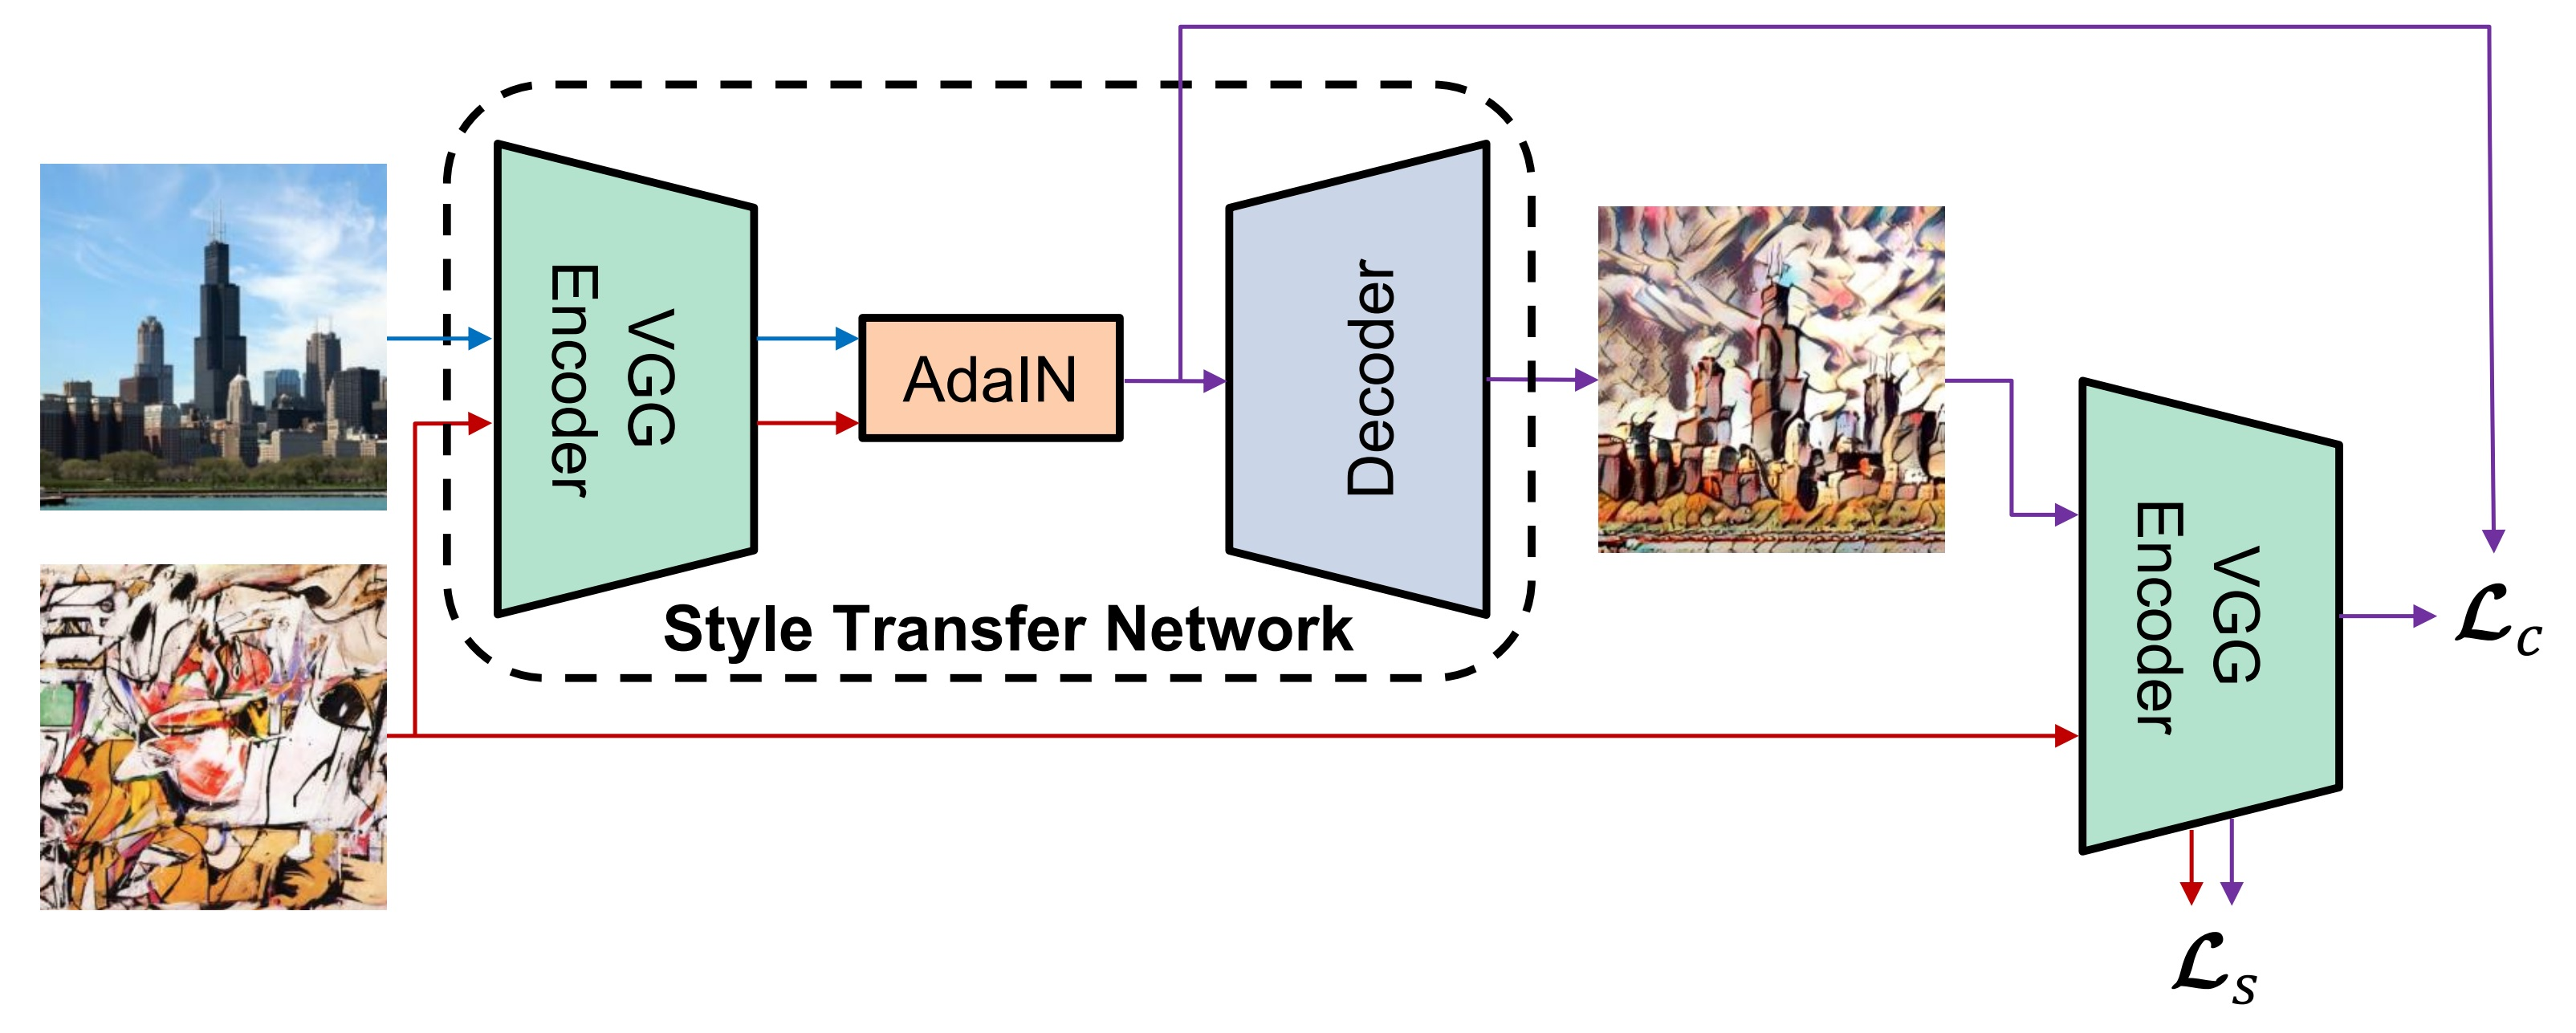
\includegraphics[width=0.45\textwidth]{imgs/adain_architecture}
  \caption{AdaIn style transfer network.}
  \label{adain-archi}
\end{figure}

\newpage
\subsection{Metrics}

We decided to only use the multi-class Accuracy, as our class are balanced, and not too numerous. \medskip \par

$ Accuracy = \frac{TP + TN}{TP + TN + FP + FN}  $ \medskip \par

\noindent
where TP is the True Positives, TN is True Negatives, FP is the sum of the False Positives
and FN is the sum of False Negatives. \medskip \par

\noindent
Top-k accuracy is a useful metric when there is a lot of classes to predict. Our dataset only
contains 10 classes, so we deemed it wasn't necessary to introduce this metric.

\subsection{ResNet}

TODO

\subsubsection{Loss Function}

\subsubsection{Optimisation Function}


\subsection{Other models ???}

TODO MAYBE ?

\subsection{Cue Conflict ???}

TODO MAYBE ?

\newpage
\section{Experiments}

For all of our experiments, SIN and IN represent Stylized-Imagenette-160 and Imagenette-160 datasets respectively.
For example, the nomenclature IN \texorpdfstring{\textrightarrow} .IN signifies that the 
model was trained on IN and tested on IN.
The two datasets have the same image identifiers for their testing set, only the stylization introduced a change.

\subsection{Texture bias hypothesis}

The first experiment conducted by the authors was to validate the texture bias 
through image classification on handpicked stylized subsets. 
Their hypothesis was that the re-texturized image would be classified as the texture representation, rather than 
the underlying content using the shapes, which would be contrary to popular belief. \medskip \par

\noindent
We've reproduced their experiment using the picture of an English Springer as our content image (a), 
and a stylized version of the Springer (b) using AdaIN style transfer
(Huang \& Belongie, 2017) described in section \ref{2.2-style-transfer}
to introduce a texture-shape cue conflicts.
The texture used to generate the stylized image is a colorful parachute, 
which can be seen in Fig. \ref{imagenette-160-parachute-predictions}. 
The model trained on imagenette-160 succesfully identified both the texture and the test image.
\medskip \par

\begin{center}
  \captionsetup{type=figure}
  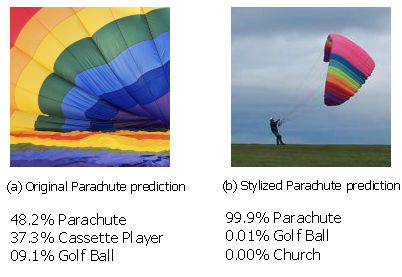
\includegraphics[width=0.35\textwidth]{imgs/experiment-1/imagenette-160-parachute-predictions}
  \captionof{figure}{Classification results of the colorful parachute texture and test image after training on imagenette-160.}
  \label{imagenette-160-parachute-predictions}
\end{center}

\noindent
The classification results after training the resnet-18 on the imagenette-160 dataset 
can be seen on Fig. \ref{imagenette-160-dog-predictions}.
We've obtained probabities in line with what was suggested by the authors, 
where the stylized image was recognized as a parachute, 
due to the texture bias, rather than an English Springer. \medskip \par

\begin{center}
  \captionsetup{type=figure}
  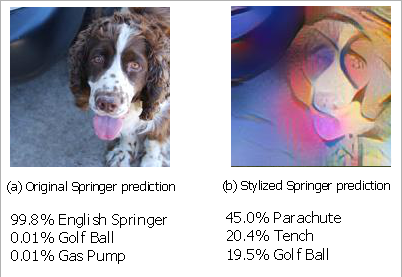
\includegraphics[width=0.35\textwidth]{imgs/experiment-1/imagenette-160-dog-predictions}
  \captionof{figure}{Classification results for the English Springer after training the model on imagenette-160.}
  \label{imagenette-160-dog-predictions}
\end{center}

\noindent
Coincidentally, training the model on the stylized dataset, 
which was believed to reduce the texture bias in favor of a shape bias, no longer produce correct predictions
for the texture image of the parachute, 
as can be seen in Fig. \ref{stylized-imagenette-160-parachute-predictions}. 
The texture image is wrongfully predicted as a garbage truck, 
due to the lack of shape clue in the image. \medskip \par

\noindent
The content image on the right however is correctly predicted, thanks to its form. 
It is also to be noted that the confidence in this prediction is lower than for the imagenette-160 trained model,
as priving the CNN from its texture bias reduce the performances of the model. \medskip \par

\begin{center}
  \captionsetup{type=figure}
  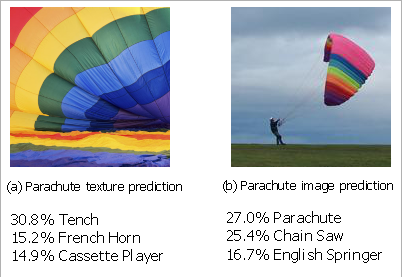
\includegraphics[width=0.35\textwidth]{imgs/experiment-1/stylized-imagenette-160-parachute-predictions}
  \captionof{figure}{Classification results of the colorful parachute texture 
            and test image after training on stylized-imagenette-160.}
  \label{stylized-imagenette-160-parachute-predictions}
\end{center}

\noindent
Retraining the model on the stylized imagenette-160 dataset with the same parameters 
(resnet-18, 20 epochs, 2e-2 learning rate), 
led to classification probabities available in 
Fig. \ref{stylized-imagenette-160-dog-predictions}. \medskip \par

\noindent
As expected, and although the results are a bit less accurate than on the original model, 
we get the correct class prediction for the stylized image, suggesting that our CNN recognized the object
from its shape this time around, having no texture clue to learn from. \medskip \par

\noindent
The confidence level for the prediction of the original image however is higher for this model, 
suggesting that it was easier to infer the class of this particuliar image 
from its shape rather than its texture. 
This shows that, although stylized-imagenette-160 does not perform on average better than imagenette-160,
there are still instances where it can out-performs the later, when enough shape clue is present. \medskip \par

\begin{center}
  \captionsetup{type=figure}
  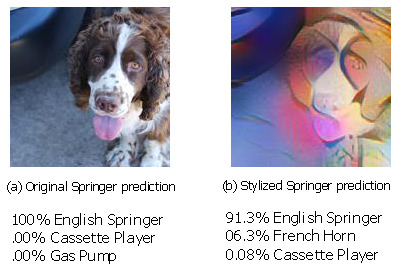
\includegraphics[width=0.35\textwidth]{imgs/experiment-1/stylized-imagenette-160-dog-predictions}
  \captionof{figure}{Classification results for the English Springer after training the model on stylized imagenette-160.}
  \label{stylized-imagenette-160-dog-predictions}
\end{center}

\noindent
The results of this experiment are also available under the dog-parachute-experiment notebook, 
in the github repository.

\newpage
\subsection{Training Procedure}


\subsubsection{Global Parameters}

\textit{Number of epochs}: For our experiments, we did a fixed number of epochs
 (15) because it did not overfit, nor underfit the data too much (Fig. \ref{loss_in}).

 \begin{figure}[h!]
  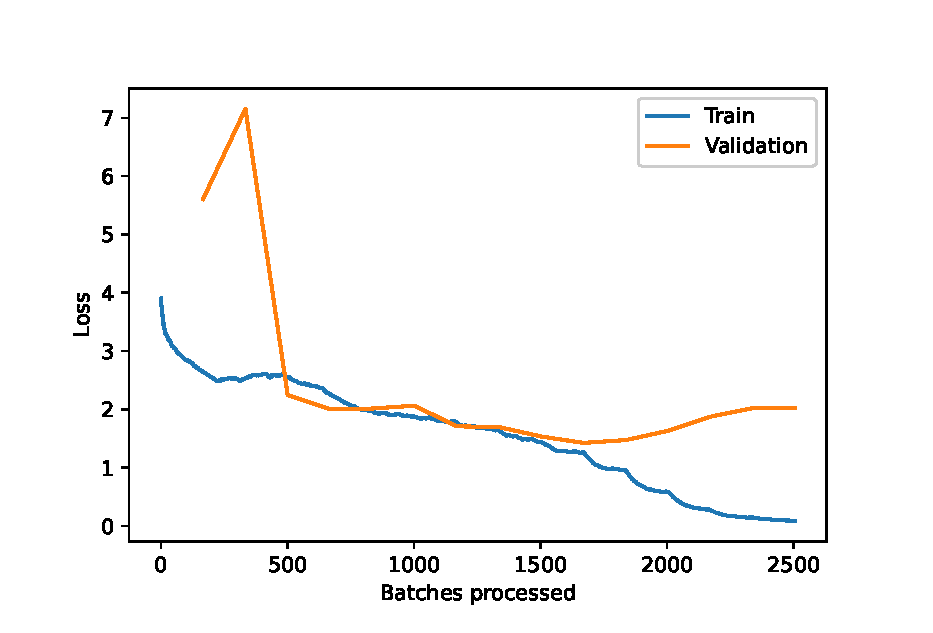
\includegraphics[width = 0.45\textwidth]{imgs/sin/loss}
  \caption{Loss of training on IN \texorpdfstring{\textrightarrow} .IN}
  \label{loss_in}
\end{figure}

\textit{Learning rate}: We used FastAI's "lr finder" (Fig. \ref{lr_finder}) to tune our learning rate.
We fixed the maximum learning rate at 1e-2 by looking at the learning rate space search graph.
\begin{figure}[h!]
  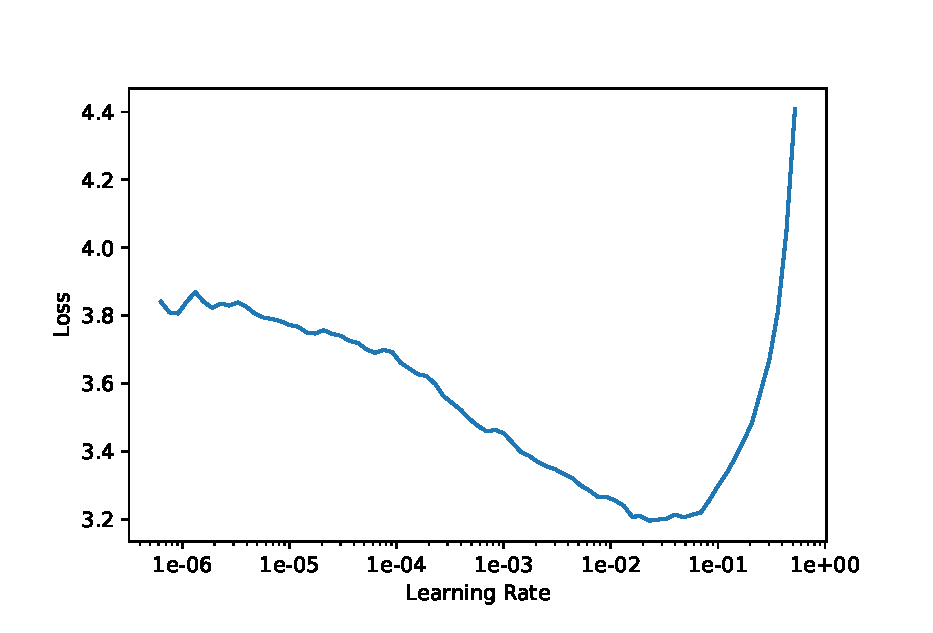
\includegraphics[width = 0.45\textwidth]{imgs/lr_find.eps}
  \caption{Learning rate finder IN \texorpdfstring{\textrightarrow} .IN}
  \label{lr_finder}
\end{figure}

\textit{Validation set}: We do a random 80/20 split of the train set to generate the 
validation set.

\subsubsection{Experiment-specific parameters}
We used an Early Stopping callback for the FineTuning experiment only, because this model was more prone to overfitting.
As we can see in Fig. \ref{lr_finetune} , the maximum learning rate has to be much lower than previous experiments 
We defined the max learning rate at 1e-4.

\begin{figure}[h!]
  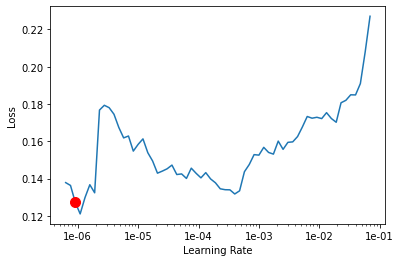
\includegraphics[width = 0.45\textwidth]{imgs/lr_finetune.png}
  \caption{Learning rate finder of SIN + IN + finetune(IN)\texorpdfstring{\textrightarrow} .IN}
  \label{lr_finetune}
\end{figure}


\subsection{Robustness of shape-based representations}

We reproduce the 4 experiments of the original paper to prove the robustness of a shape-biased CNN
(the CNN trained on SIN),
and show the fragility of the texture biased CNN (the CNN trained on IN). 

\begin{table}[h!]
  \begin{tabular}{lllll}
  \Xhline{2\arrayrulewidth}
  Architecture & IN\texorpdfstring{\textrightarrow} .IN & SIN\texorpdfstring{\textrightarrow} .SIN & IN\texorpdfstring{\textrightarrow} .SIN & SIN\texorpdfstring{\textrightarrow}.IN \\ \hline
  ResNet-18    & \textbf{0.963}     & 0.908      & 0.313     & 0.624     \\ \Xhline{2\arrayrulewidth}
  \end{tabular}
  \caption{Accuracies of ResNet18 model on different tests}
\end{table}


\subsubsection{IN \texorpdfstring{\textrightarrow} .IN}
A model trained on IN and tested on IN is the usual training scheme used in the literature.
It yields competitive results, as we already know (Fig. \ref{cm_in-in}).

\begin{figure}[h!]
  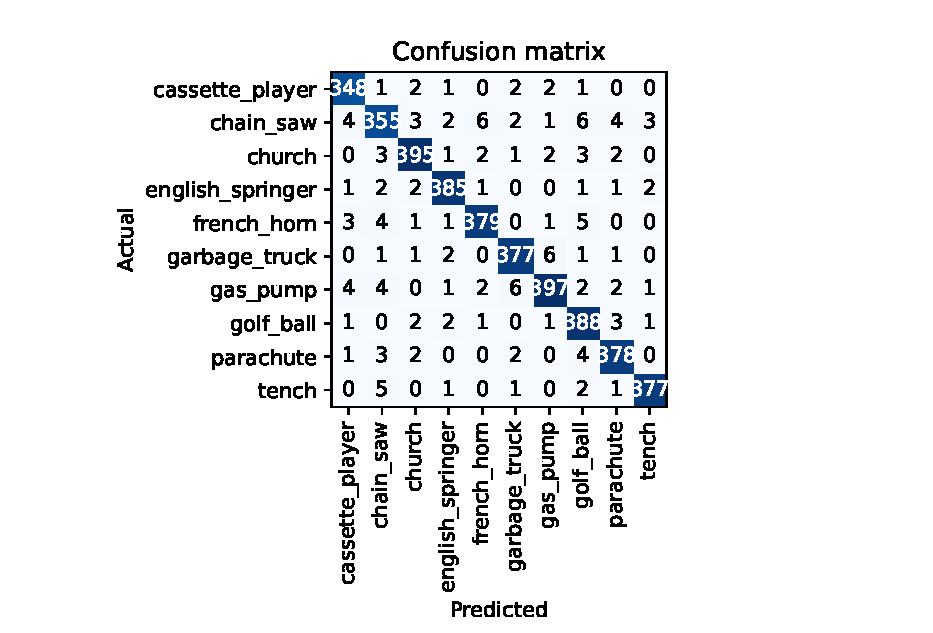
\includegraphics[width = 0.45\textwidth]{imgs/in/in-in/in-in_confusion_matrix_0.963.eps}
  \caption{Confusion Matrix of IN \texorpdfstring{\textrightarrow} .SIN}
  \label{cm_in-in}
\end{figure}

\subsubsection{IN \texorpdfstring{\textrightarrow} .SIN}



The original paper trained a model on IN and tested it on SIN which yielded poor results (Fig. \ref{cm_in-sin}) as 
the model is texture biased, and the SIN dataset is specifically designed to promote shape biased models.

\begin{figure}[h!]
  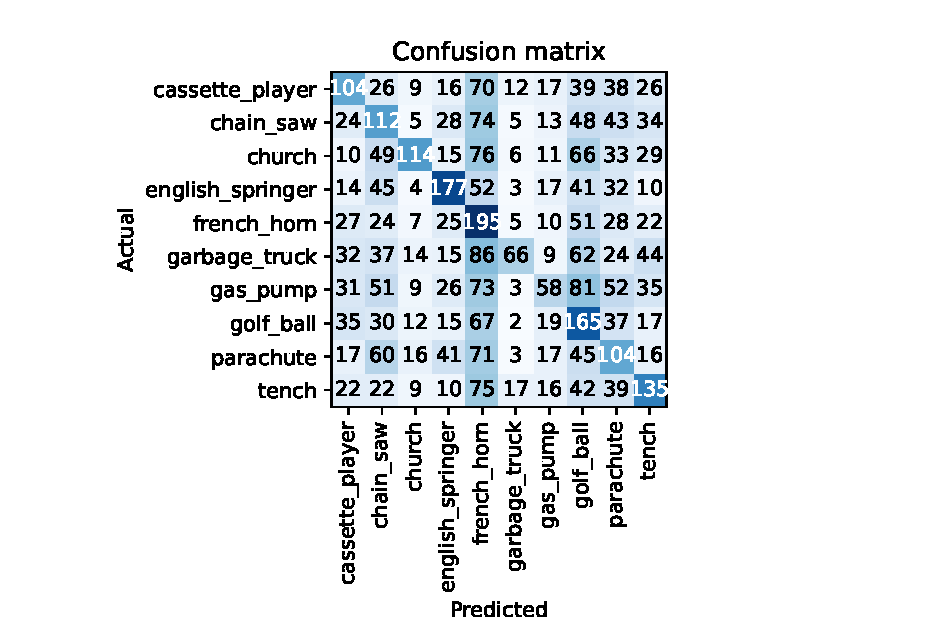
\includegraphics[width = 0.45\textwidth]{imgs/in/in-sin/in-sin_confusion_matrix_0.313.eps}
  \caption{Confusion Matrix of IN \texorpdfstring{\textrightarrow} .SIN}
  \label{cm_in-sin}
\end{figure}

\subsubsection{SIN \texorpdfstring{\textrightarrow} .SIN}
This training scheme yields fairly good results (Fig. \ref{cm_sin-sin}). This shows that the model is capable to learn
meaningful features on the stylized dataset.

\begin{figure}[h!]
  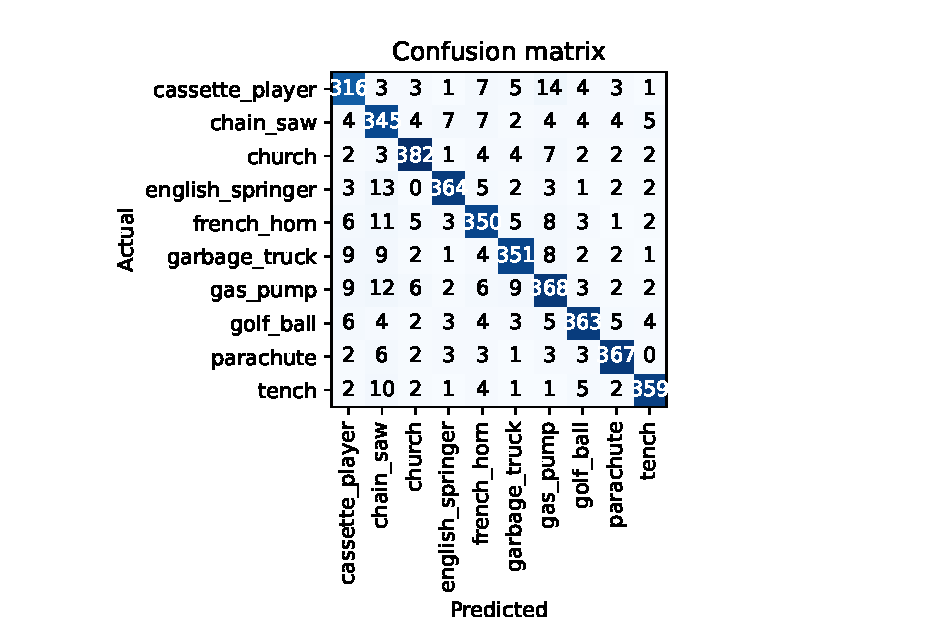
\includegraphics[width = 0.45\textwidth]{imgs/sin/sin-sin/sin-sin_confusion_matrix_0.908.eps}
  \caption{Confusion Matrix of SIN \texorpdfstring{\textrightarrow} .SIN}
  \label{cm_sin-sin}
\end{figure}

\subsubsection{SIN \texorpdfstring{\textrightarrow} .IN}

This training scheme yields superior results (Fig. \ref{cm_sin-in}) than IN \texorpdfstring{\textrightarrow} .SIN (Fig. \ref{cm_in-sin}), however
there are much better than IN \texorpdfstring{\textrightarrow} .SIN.
This demonstrates that a shape-biased model generalizes better than texture biased models.

\begin{figure}[h!]
  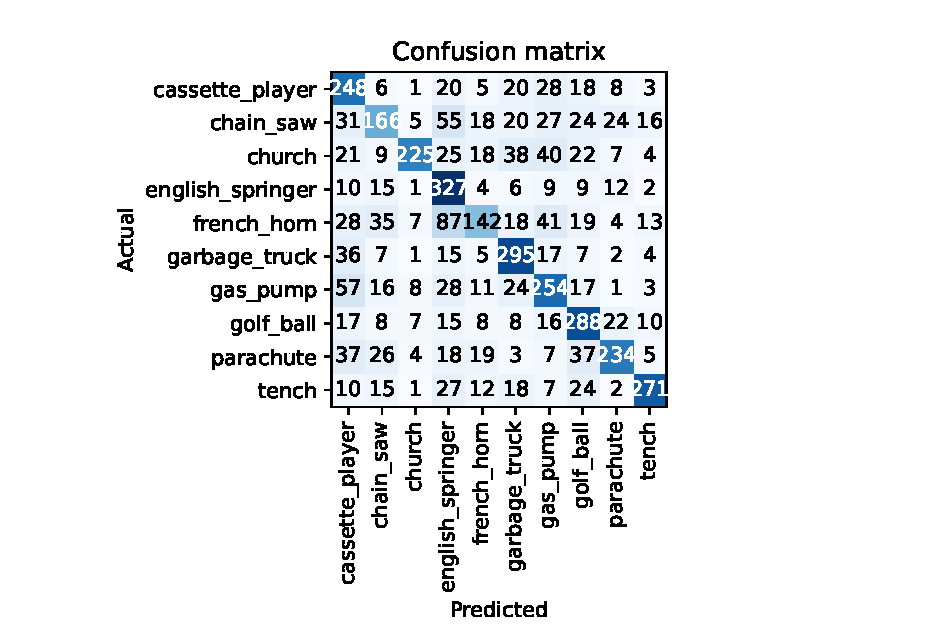
\includegraphics[width = 0.45\textwidth]{imgs/sin/sin-in/sin-in_confusion_matrix_0.624.eps}
  \caption{Confusion Matrix of SIN \texorpdfstring{\textrightarrow} .IN}
  \label{cm_sin-in}
\end{figure}

\subsection{Shape-ResNet}

Now that we demonstrated the excellent generalization capabilites of shape biased models,
our goal is to surpass the performance of the IN \texorpdfstring{\textrightarrow} .IN model.
\textbf{All the following models are evaluated on the IN test set.}

\begin{table}[h!]
  \begin{tabular}{lllll}
  \Xhline{2\arrayrulewidth}
  Architecture & IN & SIN+SIN  & SIN + IN + finetune(IN) \\ \hline
  ResNet-18    & 0.963    & 0.973   & \textbf{0.974}    \\ \Xhline{2\arrayrulewidth}
  \end{tabular}
  \caption{Accuracies of ResNet18 model on IN test set}
\end{table}


\subsubsection{SIN + IN \texorpdfstring{\textrightarrow} .IN}

Mixing the 2 datasets has the effect of a data augmentation. The model will be better
at generalizing (Fig. \ref{cm_sinin-in}). The performance improvement as a result of data augmentation 
is well known. However, this data augmentation is dedicated to increase shape bias,
and does not make the model overfit.

\begin{figure}[h!]
  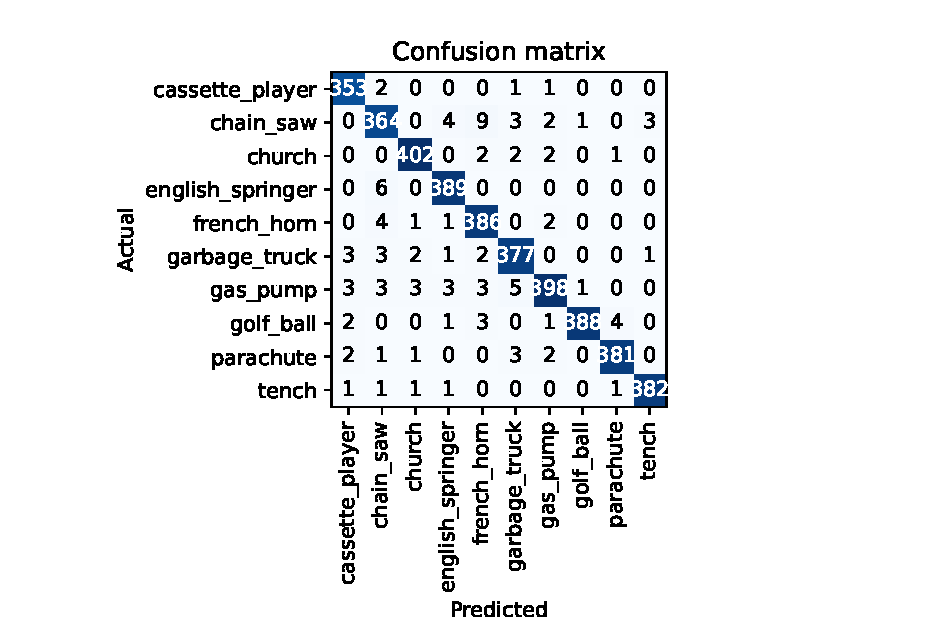
\includegraphics[width = 0.45\textwidth]{imgs/sinin/sinin-in_confusion_matrix_0.973.eps}
  \caption{Confusion Matrix of SIN + IN \texorpdfstring{\textrightarrow} .IN}
  \label{cm_sinin-in}
\end{figure}

In the Fig. \ref{loss_sinin}, we observe that the validation loss is much higher than the training
loss. The model overfits a lot on the training data.


\begin{figure}[h!]
  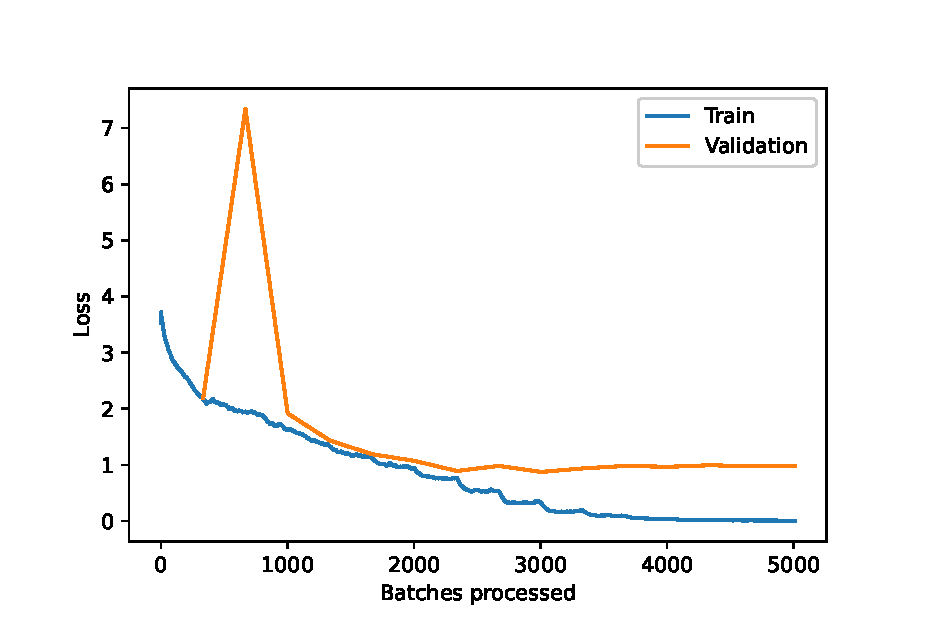
\includegraphics[width = 0.45\textwidth]{imgs/sinin/loss.eps}
  \caption{Loss of training on the SIN + IN \texorpdfstring{\textrightarrow} .IN experiment}
  \label{loss_sinin}
\end{figure}

\subsubsection{SIN + IN + finetune(IN) \texorpdfstring{\textrightarrow} .IN}

This method yields the best results (Fig. \ref{cm_sinin-in-finetune}) The finetuning only occurs
on the last layers of the ResNet (the classification layers) and not the feature extracting layers.
Hence, the model does not overfit on textures, but is better to better classify images.

\begin{figure}[h!]
  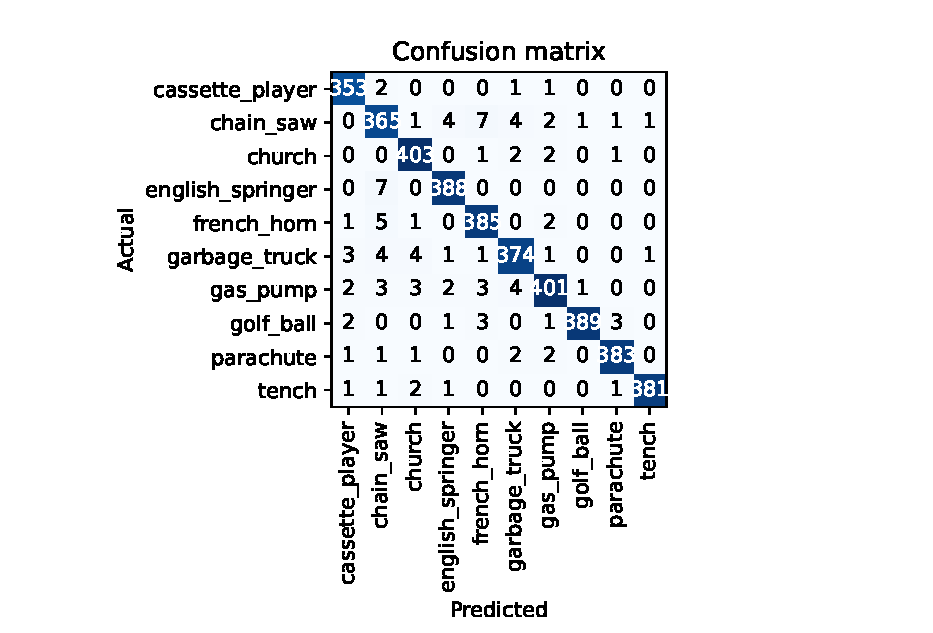
\includegraphics[width = 0.45\textwidth]{imgs/sinin/finetune/fine_tune_confusion_matrix_0.974.eps}
  \caption{Confusion Matrix of SIN + IN + finetune(IN) \texorpdfstring{\textrightarrow} .IN}
  \label{cm_sinin-in-finetune}
\end{figure}



We can see on the Fig. \ref{loss_finetune} that the train loss is fluctuating a lot even with a small
learning rate. However, the validation loss is stable and slowly decreasing.
The validation loss is slightly lower than the training loss, which is a sign of underfitting. This is what we want:
the feature extraction is more shape biased than texture biased, and the model is not overfitting on the texture like
before.
We also observe that both losses are both really low compared to the previous experiments. 
We can conclude that finetuning had a positive effect on the generalization power of the model.

\begin{figure}[h!]
  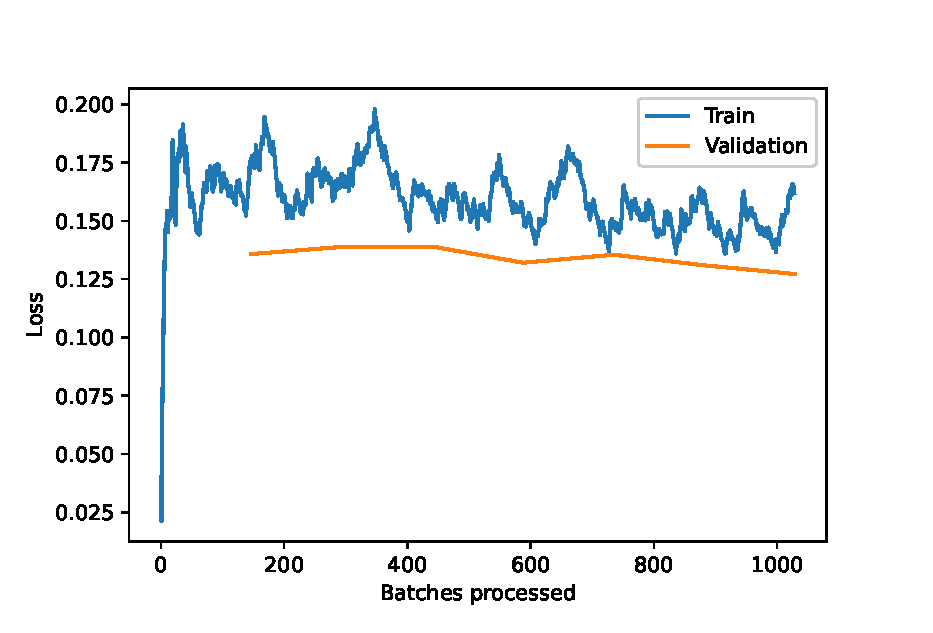
\includegraphics[width = 0.45\textwidth]{imgs/sinin/finetune/loss.eps}
  \caption{Loss of training on the finetuning experiment}
  \label{loss_finetune}
\end{figure}

\subsection{Noise resistance}


One of the major finding in the original paper was that the model trained with a shape bias had developed a better resistance to distortions than the regular model.
A model trained to recognize textures should behave differently from one trained to recognize shapes on a noised data set.  The key idea is that not all types of distortions are the same and this model should in theory only be resistant to some of them.  We decided to focus on 3 main types of distortions.  A uniform noise, a high pass filter and a low pass filter.

The result of the original paper show us that the SIN model has a better resistance to uniform noise, high pass filtered image and a worse resistance to low pass filtered images.
This makes sense since a uniform noise has a much worse effect on texture than overall shape. Also, a high pass filter acts as a contour amplifier thus making the shape in the image more prominent. In the same line of thought, a low pass filter has the opposite effect, blurring the edges of an image and making it's shape much less discernible.

\begin{figure}[h!]
\centering
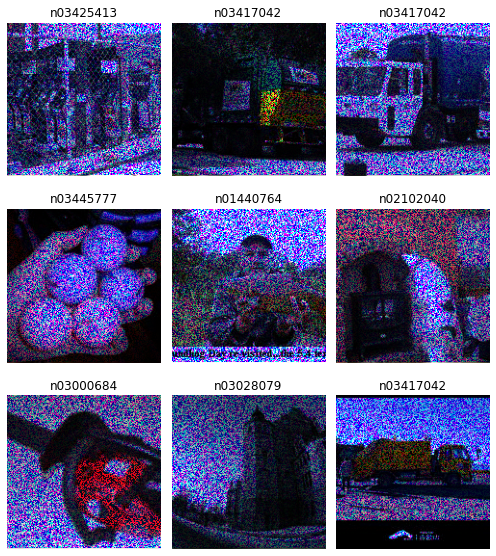
\includegraphics[width = 0.4\textwidth]{imgs/image_uniform}
\caption{Uniform noise}
\end{figure}

\begin{figure}[h!]
\centering
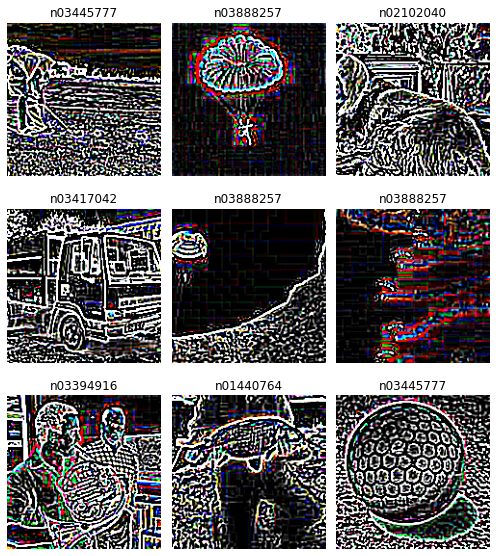
\includegraphics[width = 0.4\textwidth]{imgs/image_high}
\caption{High pass}
\end{figure}

\begin{figure}[h!]
\centering
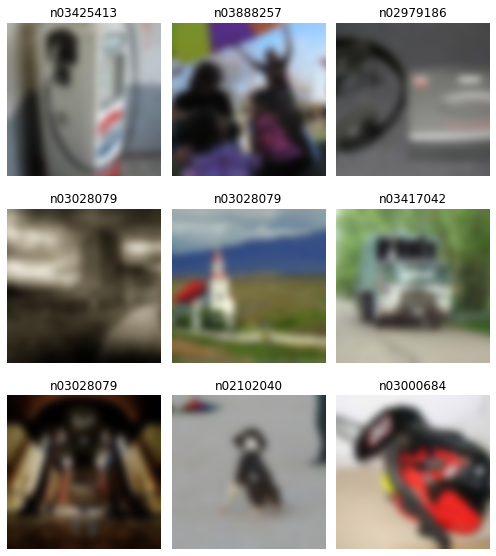
\includegraphics[width = 0.4\textwidth]{imgs/image_low}
\caption{Low pass}
\end{figure}

\subsubsection{Experiment}

We decided to reproduce this experiment with our own data.
All of the distorted data sets are created form the regular Imagenette data set. We applied the distortions at different scale gradually increasing the effect on the images.

We then compared the results of our three trained models against those different noise levels.
The models were the regular resnet trained on imagenette (IN), a resnet trained on a stylised version of imagenette (SIN) and one trained on a combination of this data (SIN+IN).
Each model was given the same test set on which a gradually increasing noise was applied and an accuracy was computed.

The different levels of noise were chosen arbitrarily to create different enough distortions. The original values and algorithms used in the paper were not available.

\subsubsection{Results}

In all of the test we conducted, the SIN model always start off worse. This is to be expected because it was trained on stylized images 
and the test set for the distorted images is based on regular images. The IN and SIN+IN model start at about the same accuracy.

\begin{figure}[h!]
\centering
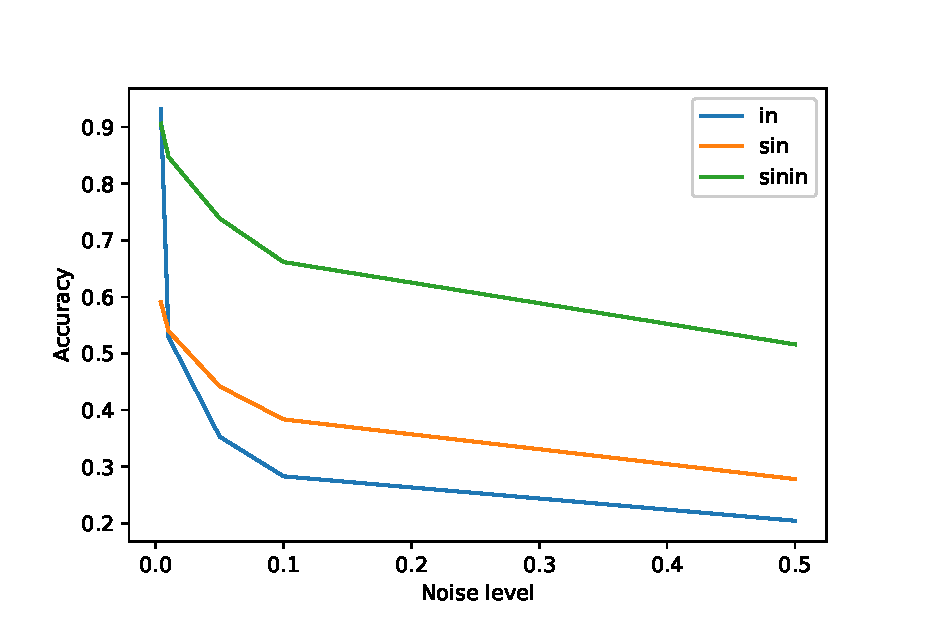
\includegraphics[width = 0.45\textwidth]{imgs/uniform}
\caption{Uniform noise}
\label{uniform_noise}
\end{figure}

\begin{figure}[h!]
\centering
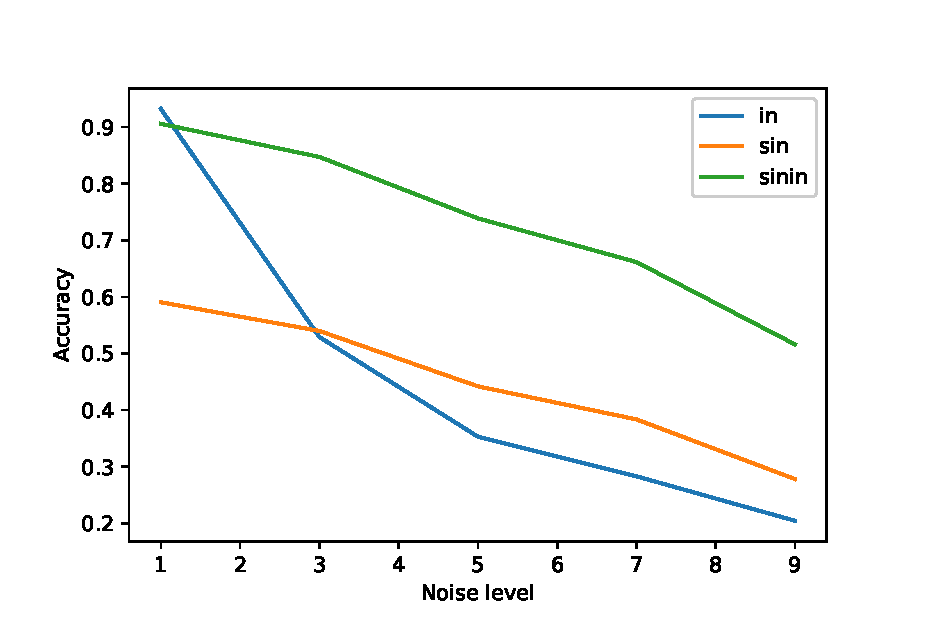
\includegraphics[width = 0.45\textwidth]{imgs/high_pass}
\caption{High pass}
\label{high_pass}
\end{figure}

\begin{figure}[h!]
\centering
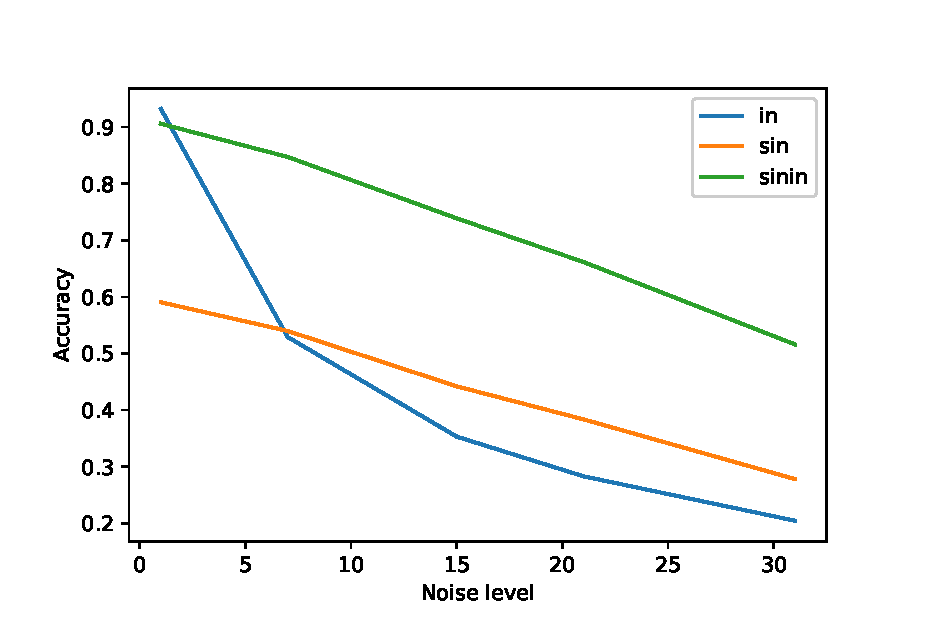
\includegraphics[width = 0.45\textwidth]{imgs/low_pass}
\caption{Low pass}
\label{low_pass}
\end{figure}

The figures clearly show the shape biased models have a better resistance to noise the regular model.

We were surprised by the results for two reasons.
First, the SIN model started off at a worse accuracy, so we were expecting to compare the resistance to distortions as a relative drop from the original accuracy but it managed to have a better absolute accuracy than the regular model.
Secondly, we were expecting the SIN model to under perform in the low pass area (Fig. \ref{low_pass}), but it managed to be better than the IN model. 
This goes against the results of the original paper and against common sense. 
It is possible the levels of blur applied were too strong for the IN model to detect any texture.

\section{Approach analysis}

The original scope of our project was to try to reproduce the findings in the reference paper.
We approached the subject with goal of of validating a simple thesis. Models can be induced with a shape bias during their training by changing the input data and this shape bias can have numerous advantages.
We would like to think that we achieved this goal, but there were some shortcomings in our methods that may have impacted our results and we would like to clarify their causes and possible effects.

\subsection{Experiments}

The first liberty we took was to only replicate a subset of the experiments of the paper.
We can see the excellent quality of the work, 
because their experiments were easily reproducible, and most of the 
steps were clearly explained.
Some of the experiment in the original paper were purely exploratory and we felt did not contribute our main thesis. As an example, we did not choose to test if human vision had an inherent shape bias as it has been a widely idea and outside our scope. \medskip \par

\noindent
Also, a lot of the experiments comparing the models against transformed test sets used transformations that we felt were a bit redundant. Some of these transformations like a silhouette detector and a gray scale version of the image were not as important as the different disturbances we introduced.
We don't feel like omitting to reproduce these experiments weakened our thesis.\\

\subsection{Dataset}

Most of the experiments depend on comparing two identical models trained on two versions of the same data set. One version left intact and another that saw stylised using the AdaIn model. \medskip \par 

\noindent
This is were we took most of our liberties because of our time and resources constraints.
The data set we chose to use for was Imagenette, a subset of the Imagenet data set.
This data set is limited by many factors. First, the number of images is considerably inferior to imagenet. Secondly, the images have lower resolution. 160 by 160 pixels in the Imagenette variant we used. Thirdly, the data set only contains 10 classes as opposed to Imagenet who has 200. \medskip \par 

\noindent
We experimented with other data sets to solve these issues, but ended up rejecting them for various reasons. The cifar10 data set's images were too low resolutions and we found the AdaIn model could not stylise them.
The original Imagenet dataset was too voluminous and the training time was too long to enable us to experiment.
Ultimately, we stayed with Imagenette and it's limitations. \medskip \par 

\noindent
The number of images reduced out training time, but also reduced the size of the test set, thus giving us less confidence in our metrics.
The lower resolution also helped our experimentation velocity by decreasing the training time, but it may have had an effect on the resistance to noise experiment. It is possible that noise applied to low resolution images has a different effect.
The fact that we only have 10 classes was helpful when we were visualising our confusion matrices but rendered one of our metric, top k accuracy, completely, unusable. The top k accuracy was used in the original paper as the top 5 accuracy on a dataset with 200 classes. It is meaningless to have a top 5 accuracy in a 10 classes dataset and reducing there is no k value for which this metric would start to be meaningful.

\subsection{Models}

The last divergence we took from the paper was our choice of models. The authors compared the effect of shape bias on 4 model architectures. Granted all of these models were slight variations of the ResNet-50, the variation of models add wight to their experiments.

In our case, we focused out training on ResNet-18. This model has a lot less parameters and is faster to train. Taking into consideration the fact that our images are of lower resolution we decided this architecture was powerful enough.

\subsection{Results}

Overall, we were able to reproduce their results and
even surpass them. This can be justified by the fact that the classes
in Imagenette were handpicked to be easily classified, and that there were less 
classes than Imagenet.
Our results fluacted a bit between different training. For example, fine tuning does not seem to be necessary 
in our study. However, when the performance of SIN + IN is sometimes lower than 0.9. In this scenario, fine tuning
always surpassed IN \texorpdfstring{\textrightarrow} .IN. \medskip \par 

\noindent
To correct this, we could have calculated our accuracy on the average of five runs, like the authors of Imagenette \cite{fastai2019}
suggested.

\subsection{Ideas for future studies}

Testing this robustness in related areas where shape bias is more important than image classification, like for example in image segmentation, could prove to be quite interesting.

\newpage
\section{Conclusion}

We were able to replicate most of the experiences of the original paper and arrive at the same results.
Our experiments showed that training a network with a combination of regular and stylised images increased its classification performance and robustness to disturbances.
This show a clear advantage of models that have a strong shape bias. \medskip \par 

\noindent
This is encouraging as it show that we are getting closer to understanding what is learned by out models. It's also interesting to know that we can introduce biases into our model by transforming the data we feed into it.


\newpage
\appendix

%% The file named.bst is a bibliography style file for BibTeX 0.99c
\bibliographystyle{named}
\bibliography{ijcai19}

\end{document}

